\section{Distributed Event Detection}
\label{sec-distrib}

Our initial deployment on Volc\'{a}n Tungurahua was small enough
that it was possible to transmit continuous signals from each of the
nodes. However, such an approach is not feasible for larger arrays deployed
over longer periods of time. We are planning to deploy a much larger
(approximately 30 node) sensor array on Tungurahua within the next 
8-12~months. To save bandwidth and energy, it is desirable to avoid
transmitting signals when the volcano is quiescent. In this section,
we describe a distributed event detector that only transmits
well-correlated signals to the base station.

%We had several advantages when approaching the general network triggering
%problem.  One stems from the eruption frequency of volcanos like Tungurahua,
%which are considered highly active when erupting merely dozens of times per
%day.  This event frequency allows time between events during which data
%collection and transmission can occur.  A second significant advantage we had
%was the data that we collected at Tungurahua.  Possessing a large amount of
%actual data collected at a real volcano on our hardware platform allowed us
%to test certain portions of our distributed event detector in simulation
%retaining total confidence in the results.

\subsection{Distributed Detector Design}

Our distributed detector uses a decentralized voting process to measure
signal correlation among a group of nodes.  Each node samples data
continuously at 102.4~Hz and buffers a window of acquired data while
running a local event detection algorithm.  When the local event detector
triggers, the node broadcasts a vote message. If any node receives
enough votes from other nodes during some time window, it initiates
global data collection by flooding a message to all nodes in the
network. Note that in this approach, voting uses local radio
broadcast, while data collection is initiated using a global flood.
Our expectation is that in a typical deployment, each node will 
have multiple neighbors within radio range with which it can compare
votes using local broadcast only. 

To reduce radio contention during data collection, we use a token-based
scheme for scheduling transmissions. Upon initiating global data
collection, the first node (ordered by node ID)
transmits its complete buffer of data to the base station, performing
retransmissions for any lost packets. Once the complete buffer has been
transmitted, the node broadcasts a message indicating that the next
node in the numeric sequence should transmit its buffer. If a node
does not hear the token exchange (or has failed), the base station will
flood the network with a data request after a timeout period, ensuring
forward progress.

\subsection{Local Detector Design}

Our design decouples the distributed voting scheme from the specific
local event detection algorithm used, allowing us to explore different
approaches. Figure~\ref{fig-explosion} shows a typical infrasonic
wave.  Designing a local event detector for this kind of waveform is
straightforward, although some tuning is required to minimize false
positives (which may trigger data collection for uncorrelated signals)
and false negatives (which may cause true explosions to be missed).

We have implemented two local event detectors: a threshold-based detector
and an exponentially weighted moving average (EWMA)-based detector. The
threshold detector is triggered whenever a signal rises above one
threshold, $T_\mathrm{hi}$, and falls below another, $T_\mathrm{lo}$,
during some time window $W$.  Because this detector relies on absolute
thresholds, it is sensitive to the particular microphone gain on each
node. It is also susceptible to false triggering due to spurious
signals, such as wind noise, although the voting scheme described above
mitigates this effect.

The EWMA detector calculates two moving averages with different
gain parameters, $\alpha_\mathrm{short}$ and $\alpha_\mathrm{long}$,
representing both short-term and long-term averages of the 
signal. For each ADC sample, each moving average is calculated as:
\[
\mathit{average} = \alpha \cdot \mathit{sample} + (1 - \alpha) \mathit{average}
\]
For our analysis below, we use $\alpha_\mathrm{short} = 0.05$
and $\alpha_\mathrm{long} = 0.002$.
For each new sample, the detector compares the ratio of the two
averages. If the ratio exceeds some threshold $T$ (i.e., the short-term 
average exceeds the long-term average by a significant amount), 
the detector is triggered. This detector is less affected by 
the sensitivity or bias of individual sensor nodes. Because a large
signal will cause the detector to trigger for multiple successive
samples, we suppress duplicate triggers over a window of 100~samples.

\begin{figure}[t]
\begin{center}
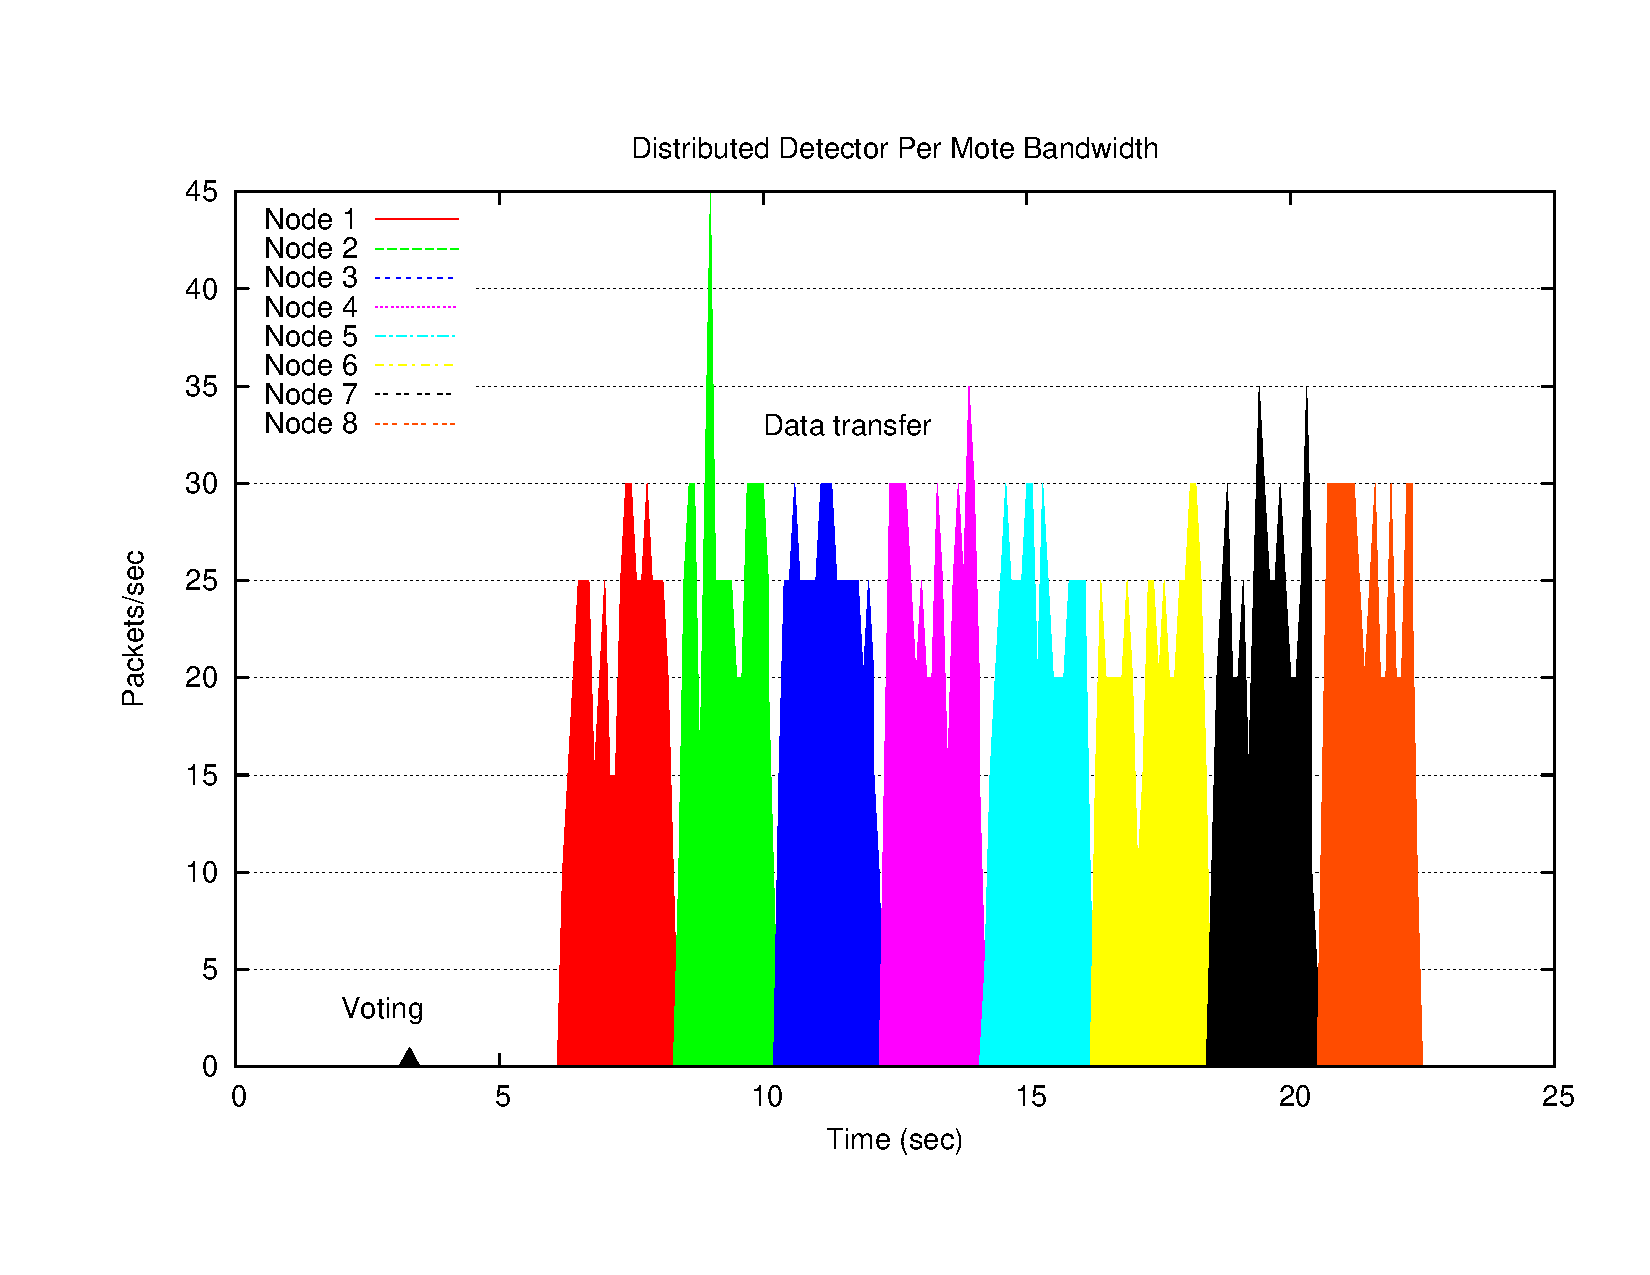
\includegraphics[width=0.9\hsize]{./figures/DD/bandwidth.pdf}
\end{center}
\caption{\small {\bf Distributed detector network bandwidth
consumption.} {\em Values are shown as packets per second. The 
voting and round-robin data collection phases are clearly visible.}}
\label{fig-packetssec}
\end{figure}

\section{Evaluation}
\label{sec-evaluation}

We implemented the distributed event detector in TinyOS and tested it
on an array of 8 Mica2 nodes in our lab.  The infrasonic signals used
to trigger the array were produced by decisively closing the lab door, 
which closely mimics infrasonic signals produced by a volcano.  Since the
lab experiments were not intended to evaluate the accuracy of the local
detector we exploited the lack of wind noise in the lab and deployed the
simple threshold detector described above.  Because we were only able
to deploy 4~nodes with infrasonic sensor boards, the voting thresholds were
adjusted accordingly.  Although only 4~nodes participated in the voting
process, data was still collected from all 8~nodes, the remaining four
equipped with standard Mica2 sensor boards (which are not sensitive 
enough to detect infrasound).

\subsection{Energy usage}

Figure~\ref{fig-continuouspowerconsumption} shows the power consumption 
of a node running the original continuous data-collection code.
For comparison, Figure~\ref{fig-ddpowerconsumption} shows the power
consumption of the distributed event detector. Each node exhibits
a baseline current draw of about 18~mA. The continuous sampling code
experiences spikes up to 36~mA during radio packet transmissions
every 4~Hz, while the distributed detector only experiences these
spikes while transmitting votes and (for correlated signals) data
transmission to the base station. 

Assuming a constant 3~V supply voltage, under the continuous sampling model 
the total power consumption over a time interval $t$ is roughly:
\[
   P_c = 3 \cdot 18 + \rho_\mathrm{tx} P_\mathrm{tx}  \mathrm{mW}
\]
where $P_\mathrm{tx}$ is the power required to transmit a single
packet, and $\rho_\mathrm{tx}$ is the rate of transmission, 
approximately 4~Hz.
For the distributed detector, the power consumption is:
\[
   P_d = 3 \cdot 18 + \rho_\mathrm{vote} P_\mathrm{tx} +
     \rho_\mathrm{send} P_\mathrm{tx} n
\]
where $\rho_\mathrm{vote}$ is the local voting rate,
$\rho_\mathrm{send}$ is the rate at which correlated signals are
transmitted to the base station, and $n$ is the number of packets in the
local window to transmit. 

On the Mica2, the time to transmit a single packet is approximately
20~ms, so $P_\mathrm{tx} = 3 \cdot 20 \mathrm{ms} \cdot 36 \mathrm{mA} =
2.16$ mW. To transmit a buffer of 1500 samples with 25 samples/packet,
$n = 60$ packets.

Assuming that nodes detect a correlated signal every 1/2 hour, 
and locally vote at twice this rate (i.e., 100\% false positive event
detection), we have
\begin{eqnarray*}
  P_c &=& 3 \cdot 18 + 2.16 / 4 = 54.54 \mathrm{mW} \\
  P_d &=& 3 \cdot 18 + 2.16 / 900 + 50 (2.16 / 1800) \\
      &=& 54.062 \mathrm{mW}
\end{eqnarray*}
for a savings of 0.48 mW. Note that in both cases, power usage is 
dominated by the 18~mA baseline current consumption. By employing careful 
duty cycling of the CPU and radio in between sampling periods, energy usage
could be reduced further, and we intend to explore this as future work.
% Lifetime: (2.850 A-hours in a battery) / (Power / 3V) = # hours

\subsection{Bandwidth usage}

\begin{figure}[t]
\begin{center}
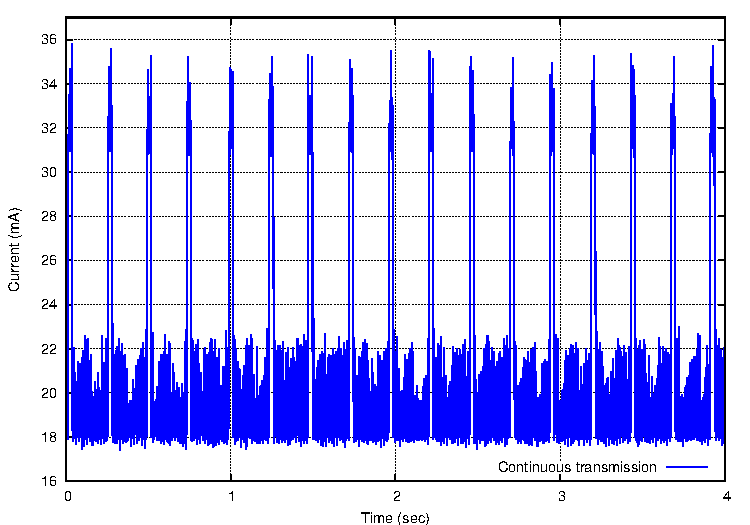
\includegraphics[width=0.9\hsize]{./figures/DD/mdw/continuous.pdf}
\end{center}
\caption{\small {\bf Power consumption of the original 
continuous data collection code.} 
{\em The baseline power consumption is about 18~mA, while
high-frequency spikes up to 22~mA are caused by ADC sampling.
The 4~Hz spikes are caused by radio 
packet transmissions. Due to CSMA backoff these transmissions
are not equally spaced.}}
\label{fig-continuouspowerconsumption}
\end{figure}

\begin{figure}[t]
\begin{center}
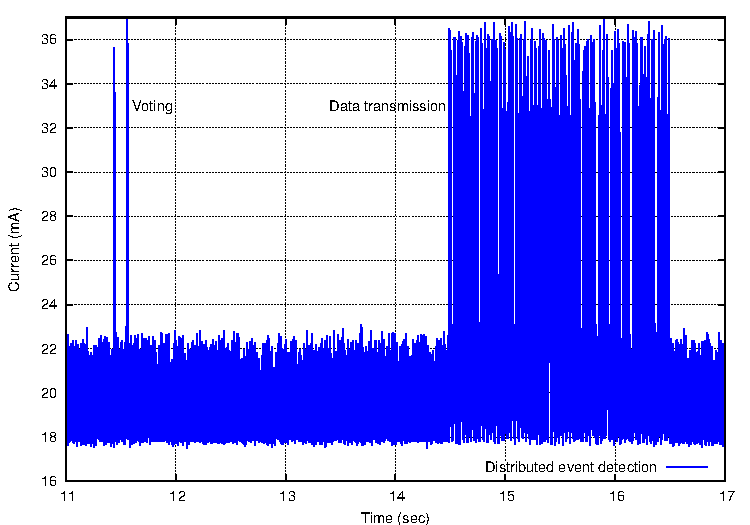
\includegraphics[width=0.9\hsize]{./figures/DD/mdw/dd.pdf}
\end{center}
\caption{\small {\bf Power consumption of the distributed event 
detection code.} {\em Overall power consumption is limited to 
sampling, while radio transmissions occur during voting and
data transfer phases.}}
\label{fig-ddpowerconsumption}
\end{figure}


Figure~\ref{fig-packetssec} shows the number of radio messages 
transmitted by the sensor array during the detection
of an event, clearly showing the voting and data collection phases.
The delay between the decision to collect data and the onset of the data
collection phase allows the nodes to center the event in their buffers.  As
shown on the graph, approximately 16~sec are required to complete data
recovery from 8 nodes in our current distributed detector. Note that we do
not currently use any compression or larger data packet sizes, 
both of which would improve transfer speed. This latency scales
linearly with the number of nodes in the array and the size of the sample
buffer on each node. The total
number of nodes in the network is bounded only by the total amount of
time to transfer complete signals to the base station, which is far
less than the expected frequency of eruptions. Even if this were not 
the case, nodes could readily log multiple events to EEPROM for later
transmission.

In contrast, the continuous sampling scheme requires each node to
transmit one packet every 1/4~sec, consuming $(n \times 4 \times 32)$
bytes/sec of bandwidth (counting application payload only), 
where $n$ is the number of nodes. 
We have benchmarked the radio performance of the Mica2 node which can
achieve roughly 7~Kbps from a single transmitter. Assuming perfect
channel sharing, a single radio hop, and no packet loss, we can optimistically 
support up to 7~nodes in this configuration. 
We have benchmarked the CC2420 802.15.4 radios on the Telos mote as 
capable of achieving about 22.5~Kbps (using the standard TinyOS MAC layer
and packet size), allowing up to 25~nodes in a single radio hop. 
However, with this many nodes it would be necessary to spread the array
over a larger area, requiring multihop communication which reduces
available bandwidth.

\subsection{Detector Accuracy}

\begin{figure*}[t]
\begin{center}
\begin{tabular}{|llllll|} \hline
{\bf Parameters} & {\em Total votes} & {\em Total events} & {\em True events} & {\em False positives} & {\em False negatives} \\ \hline
\multicolumn{6}{|c|}{\em Threshold detector} \\ 
100/900/2 & 2187 & 7 & 6 & 1 & 3 \\ 
200/800/2 & 2918 & 11 & 8 & 3 & 1 \\ 
300/700/2 & 4486 & 32 & 9 & 23 & 0 \\ 
400/600/2 & 9098 & 246 & 9 & 237 & 0 \\ \hline
100/900/3 & 2191 & 3 & 3 & 0 & 6 \\ 
200/800/3 & 2931 & 4 & 4 & 0 & 5 \\ 
300/700/3 & 4624 & 10 & 7 & 3 & 2 \\ 
400/600/3 & 11390 & 66 & 9 & 57 & 0 \\ \hline
\multicolumn{6}{|c|}{\em EWMA detector} \\ 
1.5/2 & 575 & 14 & 9 & 5 & 0 \\ 
1.75/2 & 444 & 8 & 7 & 1 & 2 \\ 
2.0/2 & 374 & 7 & 7 & 0 & 2 \\ \hline
\end{tabular}
\end{center}
\caption{\small {\bf Distributed event detector accuracy.} 
{\em For the threshold detector, the {\em Parameters} column is 
in the form {\em low/high/thresh},
where {\em low} is the low-signal threshold, {\em high} is the
high-signal threshold, and {\em thresh} is the number of nodes that
must report a local event before a correlation is made.}
For the EWMA detector, the format is {\em ratio/thresh},
where {\em ratio} is the ratio of low EWMA to high EMWA
that triggers a local event, and {\em thresh} is the voting threshold, 
as above.}
\label{fig-dd-accuracy}
\end{figure*}

The accuracy of the two local event detector algorithms is presented in
Figure~\ref{fig-dd-accuracy}. For this experiment, we fed the detectors
with the complete trace of data recorded on Tungurahua. Recall that
there are 9~known explosions in this data over a 54~hour period.
For each set of parameters, the total number of votes (potential local
events) is shown, along with the number of correlated events resulting in
global data collection. We manually verified each of the reported events
as true explosions or false positive detections.

As expected, as the local detector becomes more selective, fewer voting
rounds are initiated, although not all of the known explosions are
detected. Increasing the number of votes required to trigger global data
collection further reduces the sensitivity of the distributed detector.
It is important to keep in mind that even with a large number of false
positives, the distributed event detector saves significant bandwidth
over continuous sample transmission.


